% Created 2018-11-09 pet 08:46
% Intended LaTeX compiler: pdflatex
\documentclass[11pt]{article}
\usepackage[utf8]{inputenc}
\usepackage[T1]{fontenc}
\usepackage{graphicx}
\usepackage{grffile}
\usepackage{longtable}
\usepackage{wrapfig}
\usepackage{rotating}
\usepackage[normalem]{ulem}
\usepackage{amsmath}
\usepackage{textcomp}
\usepackage{amssymb}
\usepackage{capt-of}
\usepackage{hyperref}
\date{\today}
\title{}
\hypersetup{
 pdfauthor={},
 pdftitle={},
 pdfkeywords={},
 pdfsubject={},
 pdfcreator={Emacs 25.3.1 (Org mode 9.1.14)},
 pdflang={English}}
\begin{document}

\tableofcontents

\section{Buzzwords\hfill{}\textsc{buzz}}
\label{sec:org275d038}
\subsection{\href{https://chemistry.apache.org/project/cmis.html}{CMIS - Content Mnagement Interoperability Services}}
\label{sec:orgf7da0db}
Open standard that allows different content management systems to inter-operate over the Internet.[1] Specifically, CMIS defines an abstraction layer for controlling diverse document management systems and repositories using web protocols.
\subsection{\href{http://cifs.com/}{CIFS -Common Internet File System}}
\label{sec:orgad33872}
Network filesystem protocol used for providing shared access to files and printers between machines on the network.
\subsection{\href{https://en.wikipedia.org/wiki/JSON}{JSON - JavaScript Object Notation}}
\label{sec:org5c284ea}
An open-standard file format that uses human-readable text to transmit data objects consisting of attribute–value pairs and array data types (or any other serializable value). It is a very common data format used for asynchronous browser–server communication, including as a replacement for XML in some AJAX-style systems.[2]

JSON is a language-independent data format. It was derived from JavaScript, but as of 2017 many programming languages include code to generate and parse JSON-format data. The official Internet media type for JSON is application/json. JSON filenames use the extension .json.
\subsection{\href{https://en.wikipedia.org/wiki/Ajax\_(programming)}{AJAX - Asychronous JavaScript and XML}}
\label{sec:org6285b13}
A set of Web development techniques using many Web technologies on the client side to create asynchronous Web applications. With Ajax, Web applications can send and retrieve data from a server asynchronously (in the background) without interfering with the display and behavior of the existing page. By decoupling the data interchange layer from the presentation layer, Ajax allows Web pages, and by extension Web applications, to change content dynamically without the need to reload the entire page.[3] In practice, modern implementations commonly utilize JSON instead of XML due to the advantages of JSON being native to JavaScript.
\subsection{\href{https://www.restapitutorial.com/lessons/whatisrest.html}{REST - Representational State Transfer}}
\label{sec:org67af9a8}
Make a call from client, to server, using HTTP protocol, get response. Change "http" to "graph" in url and you get JSON (JavaScript Object Notation)  respresentation of an object.
The REST architectural style describes six constraints. These constraints, applied to the architecture, were originally communicated by Roy Fielding in his doctoral dissertation and defines the basis of RESTful-style.

The six constraints are:

Uniform Interface
Stateless
Cacheable
Client-Server
Layered System
Code on Demand (optional)

RESTful web services allow the requesting systems to access and manipulate textual representations of web resources by using a uniform and predefined set of stateless operations. Other kinds of web services, such as SOAP web services, expose their own arbitrary sets of operations.
\subsection{\href{https://en.wikipedia.org/wiki/SOAP}{SOAP - Simple Object Access Control}}
\label{sec:org964af8c}
A messaging protocol specification for exchanging structured information in the implementation of web services in computer networks. Its purpose is to induce extensibility, neutrality and independence. It uses XML Information Set for its message format, and relies on application layer protocols, most often Hypertext Transfer Protocol (HTTP) or Simple Mail Transfer Protocol (SMTP), for message negotiation and transmission.
\subsection{\href{https://en.wikipedia.org/wiki/Single\_sign-on}{SSO - Single Sign On}}
\label{sec:org444d575}
A property of access control of multiple related, yet independent, software systems. With this property, a user logs in with a single ID and password to gain access to a connected system or accomplished using the Lightweight Directory Access Protocol (LDAP) and stored LDAP databases on (directory) servers.
\subsection{\href{https://ldap.com/}{LDAP -Lightweight Directory Access Protocol}}
\label{sec:orgd451f27}
A mature, flexible, and well supported standards-based mechanism for interacting with directory servers. It’s often used for authentication and storing information about users, groups, and applications, but an LDAP directory server is a fairly general-purpose data store and can be used in a wide variety of applications.
\subsection{\href{https://en.wikipedia.org/wiki/WebDAV}{WebDAV - Web Distributed Authoring and Versioning}}
\label{sec:org3872fe8}
An extension of the Hypertext Transfer Protocol (HTTP) that allows clients to perform remote Web content authoring operations.
\subsection{\href{https://ecmarchitect.com/alfresco-developer-series-tutorials/webscripts/tutorial/tutorial.html}{Web Script}}
\label{sec:orgc455295}
Think of a web script as a chunk of code that is mapped to a human-readable URL.
\subsection{\href{https://en.wikipedia.org/wiki/Application\_programming\_interface}{API -Application Programming Interface}}
\label{sec:org3449a94}
A set of subroutine definitions, communication protocols, and tools for building software. In general terms, it is a set of clearly defined methods of communication among various components. A good API makes it easier to develop a computer program by providing all the building blocks, which are then put together by the programmer.
\subsection{\href{https://en.wikipedia.org/wiki/Software\_development\_kit}{SDK - Software Development Kit (devkit)}}
\label{sec:org4bf56a3}
A set of software development tools that allows the creation of applications for a certain software package, software framework, hardware platform, computer system, video game console, operating system, or similar development platform. To enrich applications with advanced functionalities, advertisements, push notifications, and more, most app developers implement specific software development kits. Some SDKs are critical for developing a platform-specific app. For example, the development of an Android app on Java platform requires a Java Development Kit, for iOS apps the iOS SDK, and for Universal Windows Platform the .NET Framework SDK. There are also SDKs that are installed in apps to provide analytics and data about application activity; prominent creators of these types of SDKs include Google, InMobi, and Facebook.
\subsection{\href{https://softwareengineering.stackexchange.com/questions/101873/whats-the-difference-between-an-api-and-an-sdk}{API vs SDK}}
\label{sec:org4f18e52}
It rather falls along the lines of "All SDKs are/contain APIs but not all APIs are SDKs".

An SDK seems to be a complete set of APIs that allow you to perform most any action you would need to for creating applications. In addition an SDK may include other tools for developing for the platform/item that it is for.

An API on the other hand is just a series of related methods that may be good for a specific purpose.

As an example, the JDK (Java Development Kit) contains the API as well as the compilers, runtimes, and other miscellaneous tools. The Java API is simply all the libraries that make up the core language that you can work with out of the box.
\subsection{\href{https://en.wikipedia.org/wiki/File\_Transfer\_Protocol}{FTP - File Transfer Protocol}}
\label{sec:org5afe466}
A standard network protocol used for the transfer of computer files between a client and server on a computer network.
\subsection{\href{https://en.wikipedia.org/wiki/Internet\_Message\_Access\_Protocol}{IMAP - Internet Message Access Protocol}}
\label{sec:orge42b86e}
An Internet standard protocol used by email clients to retrieve email messages from a mail server over a TCP/IP connection.
\subsection{\href{https://en.wikipedia.org/wiki/Hypertext\_Transfer\_Protocol}{HTTP - Hypertext Transfer Protocol}}
\label{sec:org89296c2}
An application protocol for distributed, collaborative, hypermedia information systems.[1] HTTP is the foundation of data communication for the World Wide Web, where hypertext documents include hyperlinks to other resources that the user can easily access, for example by a mouse click or by tapping the screen. HTTP was developed to facilitate hypertext and the World Wide Web.
\subsection{URI - Uniform Resource Identifier}
\label{sec:orgb03abb0}
\subsection{URL - Uniform Resource Locator}
\label{sec:org3b74ad4}
\section{CLI\hfill{}\textsc{cli}}
\label{sec:orgb193e43}
\subsection{Linux}
\label{sec:org5145858}
\subsubsection{Cheatsheet}
\label{sec:org312809a}
\subsubsection{General}
\label{sec:org80cdd52}
\subsection{Windows}
\label{sec:orgddf3198}
\subsubsection{Cheatsheet}
\label{sec:orgfb2becb}
\subsubsection{General}
\label{sec:org2b790c3}
\section{Git\hfill{}\textsc{git}}
\label{sec:orgada34ce}
\subsection{Cheatsheet}
\label{sec:org7e13ce6}
\subsubsection{Basics}
\label{sec:orga6d9ee9}
\begin{enumerate}
\item git init <directory>
\label{sec:org7a08c42}
Create empty Git repo in specified directory. Run with no arguments
to initialize the current directory as a git repository.
\item git clone <repo>
\label{sec:orga6549d5}
Clone repo located at <repo> onto local machine. Original repo can be
located on the local filesystem or on a remote machine via HTTP or SSH.
\item git config user.name <name>
\label{sec:org9e4ea75}
Define author name to be used for all commits in current repo. Devs
commonly use --global flag to set config options for current user.
\begin{enumerate}
\item git config --global user.name <name>
\label{sec:org0c9f948}
Define the author name to be used for all commits by the current user.
\item git config --global user.email <email>
\label{sec:org067259f}
Define the author email to be used for all commits by the current user.
\item git config --global alias. <alias-name> <git-command>
\label{sec:orge6dda8c}
Create shortcut for a Git command. E.g. alias.glog log --graph
--oneline will set git glog equivalent to git log --graph --oneline.
\item git config --system core.editor <editor>
\label{sec:org51ddcf6}
Set text editor used by commands for all users on the machine. <editor>
arg should be the command that launches the desired editor (e.g., vi).
\item git config --global --edit
\label{sec:org45f95fa}
Open the global configuration file in a text editor for manual editing.
\end{enumerate}
\item git add <directory>
\label{sec:org86c525c}
Stage all changes in <directory> for the next commit.
Replace <directory> with a <file> to change a specific file. To stage all changes for the next commit, git add . is appropriate command.
\item git commit -m "<message>"
\label{sec:org398efcb}
Commit the staged snapshot, but instead of launching a text editor,
use <message> as the commit message.
\begin{enumerate}
\item git commit --amend
\label{sec:orgcb2dc12}
Replace the last commit with the staged changes and last commit
combined. Use with nothing staged to edit the last commit’s message.
\end{enumerate}
\item git status
\label{sec:org810d387}
List which files are staged, unstaged, and untracked.
\item git log
\label{sec:orgcc03076}
Display the entire commit history using the default format.
\begin{enumerate}
\item git log -<limit>
\label{sec:orgb17bc4d}
Limit number of commits by <limit>. E.g. git log -5 will limit to 5
commits.
\item git log --oneline
\label{sec:org94d4c1f}
Condense each commit to a single line.
\item git log -p
\label{sec:org4937380}
Display the full diff of each commit.
\item git log --stat
\label{sec:org8a0d896}
Include which files were altered and the relative number of lines
that were added or deleted from each of them.
\item git log --author="<pattern>"
\label{sec:orgbf9306a}
Search for commits by a particular author.
\item git log --grep="<pattern>"
\label{sec:org2dc78a1}
Search for commits with a commit message that matches <pattern>.
\item git log <since>..<until>
\label{sec:org6fe322d}
Show commits that occur between <since> and <until>. Args can be a
commit ID, branch name, HEAD, or any other kind of revision reference.
\item git log -- <file>
\label{sec:org323206a}
Only display commits that have the specified file.
\item git log --graph --decorate
\label{sec:orga2afa6e}
--graph flag draws a text based graph of commits on left side of commit
msgs. --decorate adds names of branches or tags of commits shown.
\end{enumerate}
\item git diff
\label{sec:org9ee9524}
Show unstaged changes between your index and working directory.
\begin{enumerate}
\item git diff HEAD
\label{sec:orged3958d}
Show difference between working directory and last commit.
\item git diff --cached
\label{sec:orgf4cefbd}
Show difference between staged changes and last commit.
\end{enumerate}
\end{enumerate}
\subsubsection{Undoing Changes}
\label{sec:org8d4fb4f}
\begin{enumerate}
\item git revert <commit>
\label{sec:orgb544109}
Create new commit that undoes all of the changes made in
<commit>, then apply it to the current branch.
\item git reset
\label{sec:orgb6b8e32}
Reset staging area to match most recent commit, but leave the
working directory unchanged.
\begin{enumerate}
\item git reset <file>
\label{sec:org152aa21}
Remove <file> from the staging area, but leave the working directory
unchanged. This unstages a file without overwriting any changes.
\item git reset --hard
\label{sec:org2bd4050}
Reset staging area and working directory to match most recent
commit and overwrites all changes in the working directory.
\item git reset <commit>
\label{sec:orge59e7fa}
Move the current branch tip backward to <commit>, reset the
staging area to match, but leave the working directory alone.
\item git reset --hard <commit>
\label{sec:org49a4522}
Move the current branch tip backward to <commit>, reset the
staging area to match, resets both the staging area \& working directory to
match. Deletes uncommitted changes, and all commits after <commit>.
\end{enumerate}
\item git clean -n
\label{sec:org850abbd}
Shows which files would be removed from working directory. Use
the -f flag in place of the -n flag to execute the clean.
\end{enumerate}
\subsubsection{Rewriting Git History}
\label{sec:orgdff57a0}
\begin{enumerate}
\item git commit --amend
\label{sec:org89041ad}
Replace the last commit with the staged changes and last commit
combined. Use with nothing staged to edit the last commit’s message.
\item git rebase <base>
\label{sec:orgd955666}
Rebase the current branch onto <base>. <base> can be a commit ID,
a branch name, a tag, or a relative reference to HEAD.
\begin{enumerate}
\item git rebase -i <base>
\label{sec:orgee73026}
Interactively rebase current branch onto <base>. Launches editor to enter
commands for how each commit will be transferred to the new base.
\end{enumerate}
\item git reflog
\label{sec:org42ca3bf}
Show a log of changes to the local repository’s HEAD. Add
--relative-date flag to show date info or --all to show all refs
\end{enumerate}
\subsubsection{Git Branches}
\label{sec:orgcbb081e}
\begin{enumerate}
\item git branch
\label{sec:orgdb4bb60}
List all of the branches in your repo. Add a <branch> argument to
create a new branch with the name <branch>.
\item git checkout -b <branch>
\label{sec:org5714411}
Create and check out a new branch named <branch>. Drop the -b
flag to checkout an existing branch.
\item git merge <branch>
\label{sec:org57148f2}
Merge <branch> into the current branch.
\end{enumerate}
\subsubsection{Remote Repositories}
\label{sec:org8bf8d71}
\begin{enumerate}
\item git remote add <name> <url>
\label{sec:org173332f}
Create a new connection to a remote repo. After adding a remote,
you can use <name> as a shortcut for <url> in other commands.
\item git fetch <remote> <branch>
\label{sec:orgae05b8a}
Fetches a specific <branch>, from the repo. Leave off <branch> to
fetch all remote refs.
\item git pull <remote>
\label{sec:org0ec11bc}
Fetch the specified remote’s copy of current branch and immediately
merge it into the local copy.
\begin{enumerate}
\item git pull --rebase <remote>
\label{sec:org20098e2}
Fetch the remote’s copy of current branch and rebases it into the local
copy. Uses git rebase instead of merge to integrate the branches.
\end{enumerate}
\item git push <remote> <branch>
\label{sec:orga52f179}
Push the branch to <remote>, along with necessary commits and
objects. Creates named branch in the remote repo if it doesn’t exist.
\begin{enumerate}
\item git push <remote> --force
\label{sec:orgb3dbf97}
Forces the git push even if it results in a non-fast-forward merge. Do not use
the --force flag unless you’re absolutely sure you know what you’re doing.
\item git push <remote> --all
\label{sec:org5d27914}
Push all of your local branches to the specified remote.
\item git push <remote> --tags
\label{sec:orga0f71c4}
Tags aren’t automatically pushed when you push a branch or use the
--all flag. The --tags flag sends all of your local tags to the remote repo
\end{enumerate}
\end{enumerate}
\subsection{Install Git}
\label{sec:org104832f}
\subsubsection{Install Git on Linux}
\label{sec:orge85d1fb}
\begin{enumerate}
\item Debian / Ubuntu (apt-get)
\label{sec:orgfd7318d}
Git packages are available via apt:

\begin{enumerate}
\item From your shell, install Git using apt-get:
\begin{verbatim}
$ sudo apt-get update
$ sudo apt-get install git
\end{verbatim}

\item Verify the installation was successful by typing git --version:
\begin{verbatim}
$ git --version
  git version 2.9.2
\end{verbatim}

\item Configure your Git username and email using the following commands, replacing Emma's name with your own. These details will be associated with any commits that you create:
\begin{verbatim}
$ git config --global user.name "Emma Paris"
$ git config --global user.email "eparis@example.com"
\end{verbatim}
\end{enumerate}

\item {\bfseries\sffamily TODO} Arch
\label{sec:org7f9930e}
\item Fedora (dnf/yum)
\label{sec:org161445e}
Git packages are available via both yum and dnf:

\begin{enumerate}
\item From your shell, install Git using dnf (or yum, on older versions of Fedora):
\begin{verbatim}
$ sudo dnf install git
\end{verbatim}

or

\begin{verbatim}
$ sudo yum install git
\end{verbatim}

\item Verify the installation was successful by typing git --version:
\begin{verbatim}
$git --version
 git version 2.9.2
\end{verbatim}

\item Configure your Git username and email using the following commands, replacing Emma's name with your own. These details will be associated with any commits that you create:
\begin{verbatim}
$ git config --global user.name "Emma Paris"
$ git config --global user.email "eparis@example.com"
\end{verbatim}
\end{enumerate}
\item {\bfseries\sffamily TODO} Build Git from source on Linux
\label{sec:org7da5635}
\end{enumerate}
\subsubsection{{\bfseries\sffamily TODO} Install Git on Windows}
\label{sec:org1d1675b}
\subsubsection{{\bfseries\sffamily TODO} Install Git on Mac}
\label{sec:orgee1b3b2}
\subsection{What is Git?}
\label{sec:org01f735d}
Git is a mature, actively maintained open source project originally developed in 2005 by Linus Torvalds, the famous creator of the Linux operating system kernel. Having a distributed architecture, Git is an example of DVCS (hence Distributed Version Control System). Rather than have only one single place for the full version history of the software as is common in once-popular version control systems like CVS or Subversion (also known as SVN), in Git, every developer's working copy of the code is also a repository that can contain the full history of all changes.

\subsubsection{Performance}
\label{sec:org43cd869}
The raw performance characteristics of Git are very strong when compared to many alternatives. The algorithm implemented inside Git take advantage of deep knowledge about common attributes of real source code file trees, how they are usually modified over time and what the access patterns are. Git is not fooled by the names of the files when determining what the storage and version history of the file tree should be, instead, Git focuses on the file content itself. After all, source code files are frequently renamed, split, an rearranged. The object format of Git's repository files uses a combination of delta encoding (storing content differences), compression and explicitly stores directory contents and version metadata objects.

Being distributed enables significant performance benefits as well.

\subsubsection{Security}
\label{sec:org101acd0}
Git has been designed with the integrity of managed source code as a top priority. The content of the files a well as the true relationships between files and directories, versions, tags and commits, all of these object in the Git repository are secured with a cryptographically secure hashing algorithm called SHA1. This protect the code and the change history against both accidental and malicious change and ensures that the history is fully traceable.

\subsubsection{Flexibility}
\label{sec:org872d22b}
One of Git's key design objectives is flexibility. Git is flexible in several respects: in support for various kinds of nonlinear development workflows, in its efficiency in both small and large projects and in it compatibility with many existing systems and protocols.

Git has been designed to support branching and tagging as first-class citizens (unlike SVN) and operation that affect branches and tags (such as merging or reverting) are also stored as part of the change history.

\subsubsection{Version control with Git}
\label{sec:org3be33bc}
\begin{enumerate}
\item Git is good
\label{sec:org1ab0c9d}
Git has the functionality, performance, security and flexibility that most teams and individual developer need.

\item Git is de facto standard
\label{sec:org7a663aa}
Git is the most broadly adopted tool of its kind. Vast numbers of developers already have Git experience and a significant proportion of college graduates may have experience with only Git. In addition to the benefits of a large talent pool, the predominance of Git also means that many third party software tools and services are already integrated with Git including IDEs.

\item Git is a quality open source project
\label{sec:orgbdfc4af}
Git is a very well supported open source project with over a decade of solid stewardship. Git enjoys great community support and a vast user base. Documentation is excellent and plentiful, including books, tutorial and dedicated web sites.

\item Criticism of Git
\label{sec:org7ce8f21}
One common criticism of Git is that it can be difficult to learn. Some of the terminology in Git will be novel to newcomers and for users of other systems, the Git terminology may be different, for example, revert in Git has a different meaning than in SVN or CVS. Nevertheless, Git is very capable and provides a lot of power to its users.
\end{enumerate}
\subsection{Concepts and Benefits}
\label{sec:org31b1b2c}
Category of software tools that help a software team manage changes of source code over time. Keeps track of every modification to the code in a special kind of database. Version control protects source code from both catastrophe and the casual degradation of human error and unintended consequences.
\begin{itemize}
\item A complete long-term change history of every file. This means every change made by many individuals over the years. Changes include the creation and deletion of files as well as edits to their contents.
\item Branching and merging. Having team members work concurrently is a no-brainer, but even individuals working on their own can benefit from the ability to work on independent streams of changes. Creating a "branch" in VC tools keeps multiple streams of work independent from each other while also providing the facility to merge that work back together, enabling developers to verify that the changes on each branch do not conflict.
\item Traceability. Being able to trace each change made to the software and connect it to project management an bug tracking software such as Jira, and being able to annotate each change with a message describing the purpose and intent of the change can help not only with root cause analysis and other forensics. Having the annotated history of the code at your fingertips when you are reading the code, trying to understand what it is doing and why it is so designed can enable developers to make correct and harmonious changes that are in accord with the intended long-term design of the system. This can be especially important for working effectively with legacy code and is crucial in enabling developers to estimate future work with an accuracy.
\end{itemize}
\subsection{Git for developers}
\label{sec:orgaae69ce}
\subsubsection{Feature Branch Workflow}
\label{sec:org3a5f72d}
One of the biggest advantages of Git is its branching capabilities. Unlike centralized version control systems, Git branches are cheap and easy to merge. This facilitates the feature branch workflow popular with many Git users.

\begin{center}
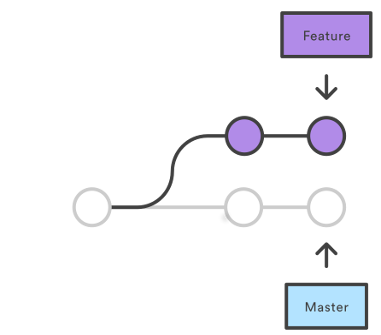
\includegraphics[width=.9\linewidth]{./img/2.png}
\end{center}

Feature branches provide an isolated environment for every change to your codebase. When a developer wants to start working on something—no matter how big or small—they create a new branch. This ensures that the master branch always contains production-quality code.

Using feature branches is not only more reliable than directly editing production code, but it also provides organizational benefits. They let you represent development work at the same granularity as the your agile backlog. For example, you might implement a policy where each Jira ticket is addressed in its own feature branch.

\subsubsection{Distributed Development}
\label{sec:org2cb7e06}
In SVN, each developer gets a working copy that points back to a single central repository. Git, however, is  distributed version control system. Instead of a working copy, each developer gets their own local repository complete with a full history of commits.

\begin{center}
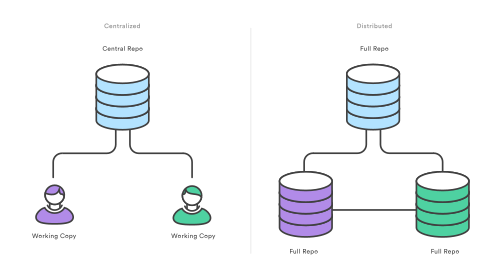
\includegraphics[width=.9\linewidth]{./img/3.png}
\end{center}

Having a full local history makes Git fast, since it means you don’t need a network connection to create commits, inspect previous versions of a file, or perform diffs between commits.

Distributed development also makes it easier to scale your engineering team. If someone breaks the production branch in SVN, other developers can’t check in their changes until it’s fixed. With Git this kind of blocking doesn’t exist. Everybody can continue going about their business in their own local repositories.

And, similar to feature branches, distributed development creates a more reliable environment. Even if developer obliterates their own repository, they can simply clone someone else’s and start anew.
\subsubsection{Pull Requests}
\label{sec:orga2bd231}
Many source code management tools such as GitHub or Bitbucket enhance core Git functionality with pull requests. A pull request is a way to ask another developer to merge one of your branches into their repository. This not only makes it easier for project leads to keep track of changes, but also lets developers initiate discussions around their work before integrating it with the rest of the codebase.

\begin{center}
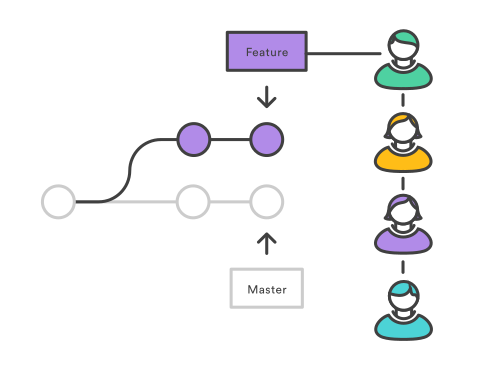
\includegraphics[width=.9\linewidth]{./img/4.png}
\end{center}

Since they're essentially a comment thread attached to a feature branch, pull requests are extremely versatile. When a developer gets stuck with a hard problem, they can open a pull request to ask for help from the rest of the team. Alternatively, junior developers can be confident that they aren't destroying the entire project by treating pull requests as a formal code review.
\subsection{Resources}
\label{sec:org349c208}
\subsubsection{Books}
\label{sec:orgfe29544}
\subsubsection{Links}
\label{sec:org58e0d6b}
\begin{enumerate}
\item \href{https://try.github.io/}{try github}
\label{sec:orgf33d95c}
\item \href{https://www.atlassian.com/git/tutorials/}{atlassian tutorials}
\label{sec:orgddfc11f}
\item \href{https://about.gitlab.com/}{about gitlab}
\label{sec:org2bd5b04}
\item \href{https://www.youtube.com/watch?v=mql6bmoysiq}{youtube}
\label{sec:orgec774a4}
\end{enumerate}
\section{Java\hfill{}\textsc{java}}
\label{sec:orga1bece1}
\subsection{Core\hfill{}\textsc{core}}
\label{sec:orgf7ae299}
\subsubsection{Resources}
\label{sec:org8c2eac1}
\begin{enumerate}
\item Books
\label{sec:org1e90b06}
\begin{enumerate}
\item \href{../notes/pdf/effectivejava2ndedition.pdf::1}{Effective Java, Second Edition}
\label{sec:orgcb401c1}
\end{enumerate}
\item Links
\label{sec:orgb11ba97}
\begin{enumerate}
\item Udemy Complete Java Masterclass
\label{sec:org56b5068}
\end{enumerate}
\end{enumerate}
\subsection{Spring\hfill{}\textsc{spring}}
\label{sec:org174ac20}
\subsubsection{Dependency injection\hfill{}\textsc{di}}
\label{sec:org6a551b3}
\begin{enumerate}
\item \href{https://en.wikipedia.org/wiki/dependency\_injection}{wiki}
\label{sec:org4c4284a}
\item \href{http://www.theserverside.com/news/1321158/a-beginners-guide-to-dependency-injection}{the serverside}
\label{sec:org415b8ca}
\item \href{http://www.vogella.com/tutorials/dependencyinjection/article.html}{vogella}
\label{sec:org0c17aa7}
\end{enumerate}
\subsubsection{Resources}
\label{sec:org7b0978b}
\begin{enumerate}
\item Books
\label{sec:org5e8a1ae}
\begin{enumerate}
\item \href{../notes/pdf/SpringInAction4thEdition.pdf::1}{Spring in Action, 4th Edition}
\label{sec:orgf520c94}
\end{enumerate}
\item Links
\label{sec:orge5dcd2d}
\begin{enumerate}
\item \href{http://docs.spring.io/spring/docs/4.0.0.RELEASE/spring-framework-reference/htmlsingle/}{Spring Docs}
\label{sec:orgad5fb44}
\item \href{https://en.wikipedia.org/wiki/Model\%E2\%80\%93view\%E2\%80\%93controller}{Wiki - MVC}
\label{sec:org4a95570}
\item \href{https://www.youtube.com/watch?v=GB8k2-Egfv0\&list=PLC97BDEFDCDD169D7}{YouTube}
\label{sec:org66fa462}
\item \href{https://www.youtube.com/watch?v=rMLP-NEPgnM}{YouTube - update}
\label{sec:org09b63a3}
\end{enumerate}
\end{enumerate}
\subsection{Maven\hfill{}\textsc{maven}}
\label{sec:org483200b}
\subsubsection{Resources}
\label{sec:orgd002838}
\begin{enumerate}
\item Books
\label{sec:org6471f3e}
\begin{enumerate}
\item \href{../notes/pdf/ApacheMaven3Cookbook.pdf::1}{Maven 3 Cookbook}
\label{sec:org976c22d}
\end{enumerate}
\item Links
\label{sec:org01a009f}
\begin{enumerate}
\item \href{https://www.tutorialspoint.com/maven/index.htm}{Tutorial Point}
\label{sec:org8076ee9}
\item \href{https://www.youtube.com/watch?v=0CFWeVgzsqY}{YouTube}
\label{sec:org391d1b2}
\end{enumerate}
\end{enumerate}
\subsection{Alfresco\hfill{}\textsc{alfresco}}
\label{sec:org4d0843e}
\subsubsection{Resources}
\label{sec:org9a96351}
\begin{enumerate}
\item Books
\label{sec:org446d397}
\begin{enumerate}
\item \href{../notes/pdf/ALFRESCO\_ONE\_5X\_DEVELOPERS\_GUIDE\_SECOND\_EDITION.pdf::23}{Alfresco One 5.x Developer's Guide}
\label{sec:org794f028}
\item \href{../notes/pdf/EdgeROIDocumentManagement.pdf::1}{Edge ROI Document Management}
\label{sec:orgc3135d3}
\item \href{../notes/pdf/ProfessionalAlfrescoPracticalSolutionsforEnterpriseContentManagement.pdf::1}{Alfresco Practical Notes}
\label{sec:org9006f92}
\end{enumerate}
\item Links
\label{sec:org9ec40f5}
\end{enumerate}
\subsection{Alfresco SDK\hfill{}\textsc{alfrescosdk}}
\label{sec:orgd4007af}
\subsubsection{Cheatsheet}
\label{sec:org83c35f7}
\begin{enumerate}
\item mvn clean install -Dmaven.test.skip=true
\label{sec:orgd45b603}
Skip tests while starting Alfresco SDK.
\end{enumerate}
\section{JavaScript\hfill{}\textsc{javascript}}
\label{sec:org888be57}
\subsection{Resources}
\label{sec:org2c58d03}
\subsubsection{Books}
\label{sec:orgb77e202}
\begin{enumerate}
\item \href{../notes/pdf/EffectiveJavaScript.pdf::1}{Effective Javascript}
\label{sec:orge2e2073}
\item \href{../notes/pdf/JavaScriptTheGoodParts.pdf::1}{JavaScript The Good Parts}
\label{sec:org441f57a}
\item \href{../notes/pdf/EloquentJavaScript.pdf::1}{Eloquent JavaScript}
\label{sec:org7537d93}
\item \href{../notes/pdf/JSDivljiZapad.pdf::1}{JS Divlji Zapd}
\label{sec:org4f33ecd}
\end{enumerate}
\subsubsection{Links}
\label{sec:org51026a8}
\begin{enumerate}
\item \href{https://www.w3schools.com/js/js\_json\_intro.asp}{w3schools - JSON}\hfill{}\textsc{json}
\label{sec:org644baf1}
\item \href{https://stackoverflow.com/questions/500431/what-is-the-scope-of-variables-in-javascript}{Scope of Variables in JS - StackOverflow}
\label{sec:orgf5908f9}
\item \href{https://developer.mozilla.org/en-US/docs/Web/JavaScript/Reference/Statements/block}{Block scoping}
\label{sec:orgf215a5b}
\end{enumerate}
\section{HTML/CSS\hfill{}\textsc{html:css}}
\label{sec:org3f1bafe}
\subsection{Tomcat\hfill{}\textsc{tomcat}}
\label{sec:orgf7a304b}
\subsubsection{\href{http://www.vogella.com/tutorials/ApacheTomcat/article.html}{Vogella Tutorial}}
\label{sec:org03aa412}
\subsection{HTTP Methods\hfill{}\textsc{httpmethods}}
\label{sec:org54687cf}
\subsubsection{\href{https://restfulapi.net/http-methods/}{RESTful API}}
\label{sec:orga8c38c6}
\subsubsection{\href{https://www.w3schools.com/tags/ref\_httpmethods.asp}{w3schools}}
\label{sec:org6ccf5e1}
\subsection{Resources}
\label{sec:org316aea4}
\subsubsection{Books}
\label{sec:orgf9c0718}
\subsubsection{Links}
\label{sec:orgf52ea0c}
\begin{enumerate}
\item \href{https://www.w3schools.com/}{w3schools}
\label{sec:org9f35092}
\end{enumerate}
\end{document}
